\documentclass[border=3mm,tikz]{standalone}

\usetikzlibrary{arrows,positioning}

    \begin{document}
	
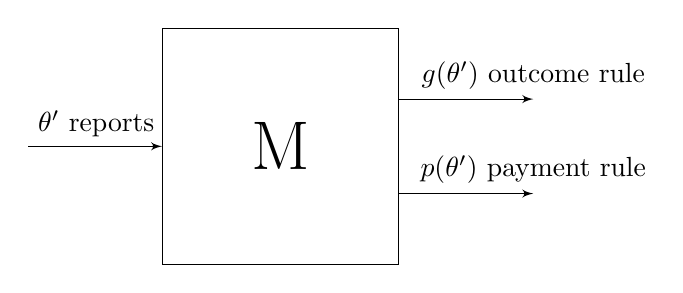
\begin{tikzpicture}[
node distance = 6mm and 17mm
                        ]
\node (m) [draw,minimum size=30mm] {\Huge{M}};

%
\coordinate[left = of m.west]   (a1);
\coordinate[above right= of m.east]  (b1);
\coordinate[below right= of m.east]  				(b2);


%
\foreach \i [count=\xi from 1] in {$\theta'$ reports}
\draw[-latex']  (a\xi) node[above right] {\i} -- (a\xi-| m.west);

\foreach \i [count=\xi from 1] in {$g(\theta')$ outcome rule ,$p(\theta')$ payment rule }
    \draw[-latex'] (m.east |- b\xi) -- (b\xi) node[above] {\i};
\end{tikzpicture}



    \end{document}